\documentclass[11pt]{article}
\usepackage[margin=1in]{geometry}
\usepackage{graphicx}
\usepackage{booktabs}
\usepackage{amsmath}
\usepackage{amssymb}
\usepackage{hyperref}
\hypersetup{colorlinks=true, linkcolor=blue, urlcolor=blue, citecolor=blue}
\usepackage{xcolor}
\graphicspath{{../figures/}}

\title{\textbf{bayanihan-net}: A Hybrid Multi-Agent System for\\
Disaster-Response Coordination under Scarcity\\[4pt]
\large An Engineering and Evaluation Study in the Marikina Flood Basin}
\author{Designing \& Building Agentic AI Systems --- Capstone}
\date{Reproducible from seed \texttt{20260620}}

\begin{document}
\maketitle

\begin{abstract}
We present \textbf{bayanihan-net}, a small but credible multi-agent system (MAS) that coordinates
scarce rescue assets during a typhoon-induced urban flood in the Marikina River basin, Metro Manila.
The system combines three coordination primitives in a defended \emph{hybrid}: a blackboard Common
Operating Picture for shared situational truth, a contract-net auction scored on \emph{global social
welfare} for scarce-asset allocation, and a command-center supervisor with a human-in-the-loop (HITL)
gate for irreversible actions. The safety-critical control plane is pure, deterministic, and fully
tested; only the disaster world is stochastic, driven by a single seed. Across twelve paired seeds, the
only policy difference clearing a 2-SE screen is the hybrid significantly outserving a \emph{random}
allocator (severity-weighted $+0.0125$); against the other reasonable policies (greedy-nearest, FIFO,
fairness ordering) the differences fall within noise, because under hard capacity saturation reachability
and capacity---not the allocation rule---are what bind. The hybrid survives a seven-scenario red-team
stress battery with zero safety-invariant violations. We
report a \emph{negative} result honestly: a fairness-weighted scheduling lever fails to improve equity
under capacity saturation because reachability, not scheduling order, is the binding constraint. Finally,
an offline reinforcement-learning routing study reproduces reward hacking---a naive travel-time reward is
beaten on the true objective by a risk-aware reward, which in turn beats the hand-coded heuristic. The
system is capacity-saturated by construction (nine assets, thousands at risk), the realistic disaster
regime; we treat the resulting modest, mostly within-noise separation between policies as a finding
rather than a defect.
\end{abstract}

\section{Introduction}
When a typhoon stalls over Metro Manila, the Marikina River rises through its alarm levels and the
low-lying barangays along it flood within hours. A small fleet of rescue boats, transport trucks, and
medical teams must be allocated across many simultaneous, evolving incidents---some unreachable at the
flood peak, some irreversible once begun. This is a problem that is distributed (no agent sees the whole
flood), specialized (triage vs.\ medical vs.\ logistics vs.\ routing), concurrent, failure-prone (a
typhoon degrades power and comms), and inter-organizational (barangay $\to$ city $\to$ NDRRMC). These are
precisely the conditions under which a \emph{single} agent is the wrong shape and a multi-agent system
must earn its keep.

Our contribution is not a new model but an \emph{engineering and evaluation study}: a working,
reproducible system with a real coordination mechanism, a real safety story, and honest failure analysis,
graded on behaviour rather than slides. All numbers below are produced by code, from a seed, with no API
key.

\section{System Design}
\paragraph{Why a hybrid.} Each coordination primitive is the right tool for one sub-problem. A
\emph{blackboard} is correct for a shared situational truth no single agent owns; it enforces idempotency
(duplicate suppression with corroboration fusion), leases/freshness (a stale-COP guard), and atomic
commitment (the single \emph{no-double-commit} chokepoint). \emph{Contract-net} is the textbook fit for
heterogeneous assets with different costs and reach: a prioritized incident triggers a call-for-proposals,
capable agents bid feasible idle assets, and the coordinator awards. A \emph{supervisor with HITL}
provides accountable arbitration and escalation for irreversible, high-stakes actions. The pure
alternatives each fail: a pure supervisor is a single point of failure (fatal here); a pure market lacks
shared awareness and escalation; pure consensus is too slow for life-safety decisions. The hybrid gives
shared awareness, efficient allocation, and accountable escalation, and it degrades gracefully.

\paragraph{Incentive alignment.} The central tension is local versus global: each logistics agent locally
wants to maximize its own utilization, while the global objective is to minimize severity-weighted unmet
harm, equitably. We resolve it structurally---\emph{the bidder does not choose the winner}. A bidder
reports a selfish local cost, but the coordinator ranks bids by a global welfare score,
\begin{equation}
W(\text{bid}) \;=\; \frac{\text{severity}\,\cdot\,\min(\text{capacity}, \text{people})}
{\text{eta}+1}\,\bigl(1 - \tfrac{1}{2}\,\text{route\_risk}\bigr),
\end{equation}
so an agent cannot win by hoarding or cherry-picking easy work; the only way to win is to be the globally
best option. This is a contract-net analogue of welfare-maximizing (VCG-flavoured) allocation.

\paragraph{Emergence as engineering.} Each unwanted emergent behaviour is named, given a metric, and
given a guardrail: asset oscillation (reassignment rate $\to$ commitment hysteresis), triage inequity
(coverage Gini / worst-served fraction $\to$ severity-first ordering), report-storm amplification (message
volume $\to$ content-key dedup), and stale-COP herding (observation freshness $\to$ leases plus
arrival-time validation against the \emph{true} flood, stranding a mis-routed asset rather than
teleporting it).

\paragraph{Interoperability.} Two real-in-code boundaries with mocked upstreams: a policy-gated
\emph{MCP} tool boundary---the PAGASA river gauge invoked every tick (48 traced calls per run), with the
MMDA-closure and DOH-bed adapters registered and scope-declared but not invoked in the current loop, all
scope-checked and trace-propagating---and an \emph{A2A} cross-agency work-exchange boundary (medical
mutual aid from a neighbouring agency, with a local access policy owned by the receiver, idempotency, and
retry).

\section{Methods}
The simulation is discrete-event over a 12-hour horizon (48 ticks). A seeded world advances the
hydrograph, floods the road graph, and emits a citizen-report stream (with duplicates and optional Sybil
injection). The control plane is deterministic; the world RNG and the engine-side RNG (comms-drop, asset
loss) are separate so injecting stress never perturbs the underlying disaster. Evaluation is two-tier:
\emph{Tier~A} invariants are a hard gate, and
\emph{Tier~B} compares the hybrid against five ablation baselines---\texttt{fairness\_weighted},
\texttt{no\_governance}, \texttt{greedy\_nearest}, \texttt{fifo}, \texttt{random}---across twelve seeds.
Comparisons are \emph{paired} by seed (hybrid minus baseline on the same world) so per-seed variance
cancels; a difference is flagged when its magnitude exceeds twice its standard error---a 2-SE
\emph{screen}, not a formal paired $t$-test (which at $n{=}12$ would use ${\approx}2.2\,\mathrm{SE}$), so
we report it as a screen and lean on consistency of sign across seeds rather than a $p$-value.
The Tier~A gate (\texttt{run\_evals.py}, non-zero exit on any violation) checks, for every
(policy, seed) cell, no-double-commit and $\text{served}\le\text{true need}$ with bounded metrics, and for
every red-team scenario, additionally serving some need (graceful degradation) and re-stabilizing.

\section{Results}
\subsection{Coordination beats no coordination; reasonable policies are within noise}
Table~\ref{tab:eval} reports per-policy means; Figure~\ref{fig:policy} visualizes them. The one
paired-significant service result is that the hybrid outserves the \emph{random} allocator
(severity-weighted $+0.0125$, raw served $+0.0136$): triage and welfare scoring earn their keep over
acting at random. Against the other \emph{reasonable} policies---greedy-nearest selection, FIFO ordering,
fairness ordering---every delta is within the 2-SE screen. Under hard capacity saturation the binding
constraint is which barangays one can physically reach with the assets on hand, not the rule by which bids
are scored or the queue is ordered; welfare scoring still \emph{directionally} lowers coverage inequality
(Gini $-0.0085$ versus greedy) and we default to it on that and on its safety properties, but we make no
significance claim where the data shows none.

\begin{table}[h]
\centering
\caption{Per-policy means over 12 paired seeds. ``sev-wt served'' is severity-weighted served fraction
(efficiency); ``worst'' is the worst-served barangay's coverage and ``cov.\ Gini'' the inequality of
coverage (equity, lower is fairer).}
\label{tab:eval}
\begin{tabular}{lcccc}
\toprule
Policy & sev-wt served & worst-served & cov.\ Gini & SLA \\
\midrule
\textbf{hybrid} & 0.353 & 0.220 & 0.109 & 0.606 \\
fairness\_weighted & 0.350 & 0.212 & 0.109 & 0.602 \\
no\_governance & 0.355 & 0.222 & 0.111 & 0.615 \\
greedy\_nearest & 0.354 & 0.217 & 0.118 & 0.606 \\
fifo & 0.348 & 0.220 & 0.106 & 0.599 \\
random & 0.340 & 0.203 & 0.113 & 0.597 \\
\bottomrule
\end{tabular}
\end{table}

\begin{figure}[h]
\centering
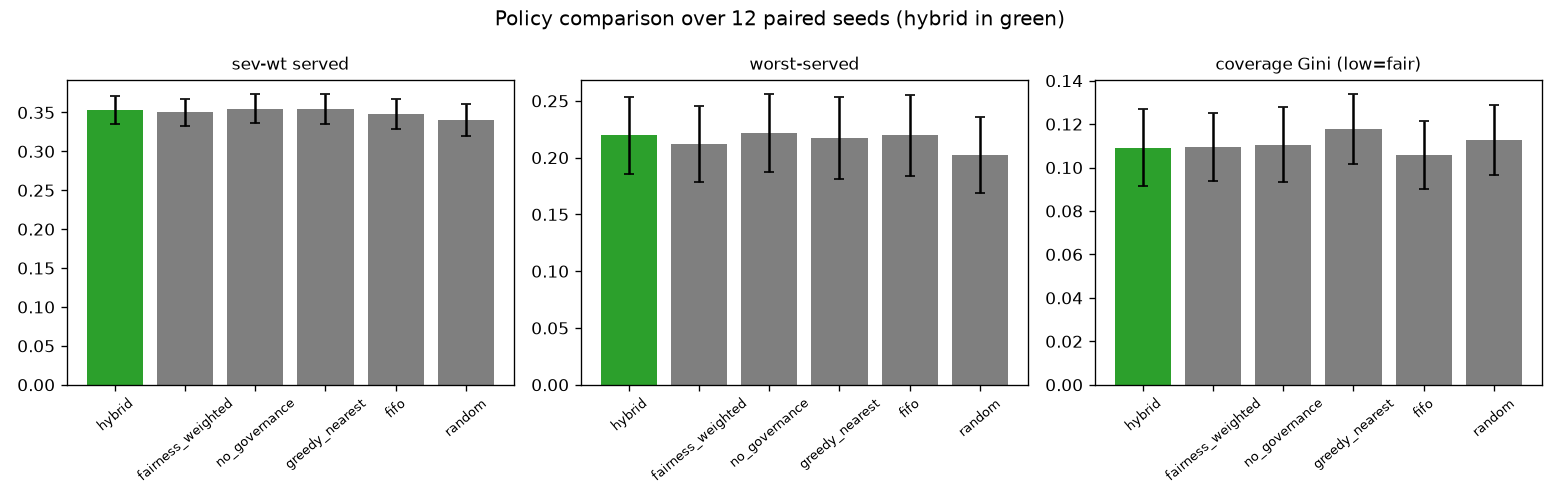
\includegraphics[width=\textwidth]{policy_comparison.png}
\caption{Policy comparison over 12 paired seeds (hybrid in green; error bars are $\pm$ one standard error).
The reasonable policies overlap within one standard error on service and equity; only the random allocator
is clearly worse, and welfare scoring is directionally the least unequal.}
\label{fig:policy}
\end{figure}

\subsection{Governance is nearly free at baseline, essential under stress}
Removing the HITL gate (\texttt{no\_governance}) changes baseline service by ${\sim}0.2$ pp---the safety
machinery costs almost nothing when nothing is wrong. Its value appears under stress: all seven red-team
scenarios (report storm, Sybil injection, comms blackout, 25\% asset loss, gauge outage, and a compound
crisis) re-stabilize with \emph{zero} safety-invariant violations. The report storm keeps service near
baseline because content-key dedup absorbs the $4\times$ duplicate flood; asset loss degrades gracefully
as leases are reclaimed and work re-auctioned.

\subsection{An honest negative: fairness scheduling does not help}
The \texttt{fairness\_weighted} variant---re-ordering the queue toward currently-under-served
barangays---is \emph{directionally worse} than the hybrid on worst-served coverage (hybrid $+0.0080$), but
within the 2-SE screen, so we make no significance claim---only that the lever fails to help.
Prioritizing the worst-off sends scarce boats to the hardest-to-reach places, where they are tied up
without lifting that community's final coverage, because the binding constraint is reachability and
capacity, not scheduling order. We keep the lever as an evaluated variant, default the system to the
better severity ordering, and report the result rather than concealing it.

\subsection{Reward hacking in the routing study}
We train two routing policies from identical dynamics but different rewards: \texttt{naive} (travel time
only) and \texttt{risk\_aware} (time plus flood-exposure penalty), then score both on a fixed
in-distribution evaluation set by a true objective the naive learner never saw (Figure~\ref{fig:rl}). The naive policy optimizes the
travel-time proxy yet loses on the true objective ($2.53$ vs.\ $2.71$) because it routes through fast,
deep water; the risk-aware policy takes less exposure and wins, and even edges out the hand-coded
risk-aware heuristic ($2.36$). This reproduces the proxy-versus-true reward gap: \emph{you get what you
reward, not what you want}. The learned policy is sandboxed and offline; in the live system the
deterministic heuristic remains the authority.

\begin{figure}[h]
\centering
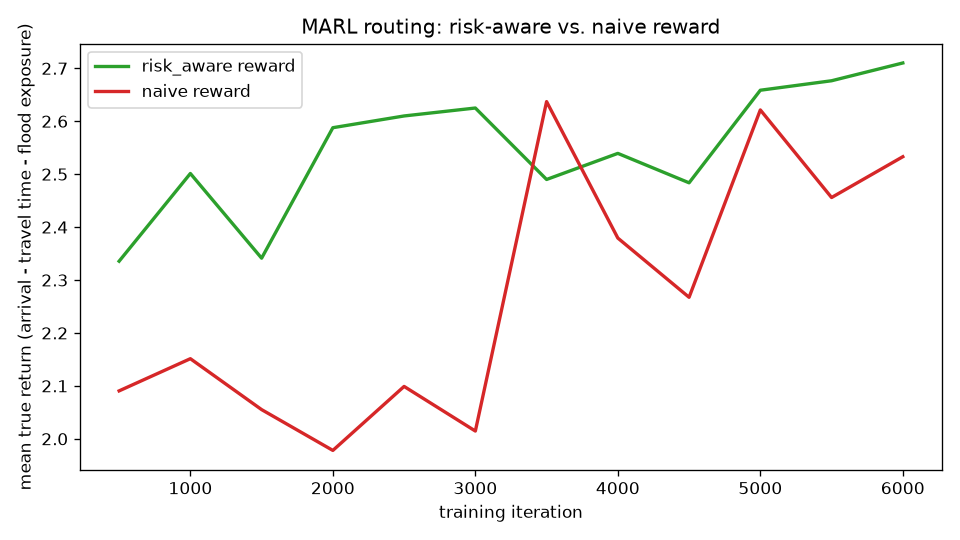
\includegraphics[width=0.85\textwidth]{rl_training_curve.png}
\caption{Offline routing study: mean true-objective return versus training iteration. The risk-aware
reward (green) pulls ahead of the naive travel-time reward (red) as training proceeds.}
\label{fig:rl}
\end{figure}

\section{Discussion and Limitations}
The system is capacity-saturated by construction---nine assets cannot serve thousands in twelve hours---so
no allocation policy can serve dramatically more people; the achievable gains are in \emph{who} is served
and \emph{how equitably and safely}. The effect sizes between the reasonable policies are therefore modest
and mostly within the 2-SE screen; the one paired-significant service result is the hybrid over the
uncoordinated (random) allocator. Known limitations, detailed in the reflection log: deduplication can merge two
genuine incidents in one barangay-window; partial service is not re-queued; the ``human'' is a
deterministic policy (good for reproducibility, not a study of real reviewer behaviour); external feeds and
partners are mocked; the RL study is tabular and weakly-coupled (CTDE via parameter sharing). The geography
is illustrative, not official Marikina data.

\section{Conclusion}
A defended hybrid MAS---blackboard, welfare-scored contract-net, and HITL supervision---coordinates scarce
disaster-response assets with provable safety invariants, graceful degradation under a stress battery, and
a paired-significant service advantage over an uncoordinated (random) allocator. An offline RL routing
study earns a bounded, advisory role and demonstrates reward hacking. The honest headline is that under
hard scarcity the reasonable allocation policies are statistically indistinguishable on service---reachability
and capacity bind, not the scoring or ordering rule---so coordination's demonstrable value is beating no
coordination at all, plus safety and graceful degradation; and a naively-added fairness lever fails to
improve equity, a result we measured, kept, and explained.

\vspace{1em}
\noindent\textbf{Reproducibility.} All results regenerate via
\texttt{python -m bayanihan\_net.cli \{run,eval,stress,rl-train\}} and
\texttt{python evals/run\_evals.py}; every artifact is stamped with seed, library versions, and an
environment fingerprint.

\end{document}
